%%% Template for AUTHOR's DRAFT paper in FCAA, WITHOUT Journal's head  %%%%%%%%%%%%%%%%%%%%%%%%%%%%%%%%%
%%% by V. Kiryakova, updated Nov. 1, 2014
%%% uses "fcaa.cls", or "fcaa-var.cls" as modifications of "amsart.cls" for the FCAA format,
%%% and auxiliary file "fcaa_style.tex" fixing page margins, fontsize, defs for theorems, proofs etc.
%%% Put the files "fcaa.cls", "fcaa-var.cls" and "fcaa_style.tex" in same directory you prepare the paper

  %\documentclass[twoside,reqno,11pt]{fcaa}  %%% or in case of problems, use as below: %
   \documentclass[twoside,reqno,11pt]{fcaa-var} %

 \input fcaa_style

%%%%%%%%%%%%%%%%%%%%
 \usepackage{hyperref} % Editor will use to create hyperlinks %
 %%% but if the author has problems with the above style file,
 %%% then comment the line \usepackage{hyperref} or replace by this below:
 % \usepackage{upref}
%%%%%%%%%%%%%%%%%%%%

% to have 2-digits numbering for equation, use:
 \def\theequation{\arabic{section}.\arabic{equation}}

%%%%%%  First page footnote for Copyright and Springer logo
 \def\themycopyrightfootnote{\vspace*{3pt}
 \copyright \, Year\,  Diogenes  Co., Sofia
   \par  \noindent pp. xxx--xxx, DOI: ......................
   \hfill  \vspace*{-36pt}
   % \mbox{\includegraphics[scale=0.65]{DeGryuter.eps}}
  }
%%%%%%%%%%%%%%%%%%%%%%%%%%%%%%%%%%%%%%%%%%%%%%%%%%%%%%%%%%%%

  \setcounter{page}{1}
  \thispagestyle{empty}

 %%%%%%%%%%%%%%% begin make title %%%%%%%%%%%%%%%%%%%%%%%%%%%%%
 %%% TITLE: texts in [.] is abbreviated (1st line) title for running heads
 %%% Author(s): put in brackets [.] the short author's name

 \title[VISUALIZATION OF FRACTIONAL INTEGRALS]{VISUALIZATION OF THE RIEMANN-LIOUVILLE FRACTIONAL INTEGRAL \\ [3pt] IN ``FCAA'' JOURNAL}
 \author[\normalsize V. Kiryakova, S. Author]{\normalsize Virginia Kiryakova $^1$, Second Author $^2$}

 %%% obligatory give the full and abbreviated authors' names %%%
 %%%%%%%%%%%%%%%%%%%%%%%%%%%%%%%%%%%%%%%%%%%%%%%%%%%%%%%%%%%%%%%
                    % THE BEGINNING %
 \begin{document}

 \vbox to 2.5cm { \vfill }

%%% to make empty space of approx. 2.5cm %%%%%%
%%% will be replaced by Editor with the journal's and publoishers logos %%%%%%%%

 \bigskip \medskip

%%%% Abstract %%%%%%%%%%%%%%%%%%%%%%%%%
 \begin{abstract}

Text of the abstract. Text of the abstract. Text of the abstract.
Text of the abstract. Text of the abstract. Text of the abstract.
Text of the abstract. It should give a comprehensive idea about the
paper's subject and the author's results. The Abstract (and the first 2 pages of the paper) will be
available free at DeGryuter's website for the journal.

 \medskip

{\it MSC 2010\/}: Primary 26A33;
                  Secondary 33E12, 34A08, 34K37, 35R11, 60G22, ...

 \smallskip

{\it Key Words and Phrases}: fractional calculus, Mittag-Leffler
type functions, fractional ordinary and partial differential
equations, ...

 \end{abstract}

 \maketitle

%%%%%%% end make title %%%%%%%%%%%%%%%%%%%%%%%%%%%%%%%%%%
 \vspace*{-16pt}

%%%%%%%% begin papers' body %%%%%%%%%%%%%%%%%%%%%%%%%%%%%

%%%%%%%%%%%%%%%%%%%%%%%%%%% Section 1 %%%%%%%%%%%%%
%\section{Introduction}\label{Sec:1}

\section{First section of the paper}\label{sec:1}

\setcounter{section}{1}
\setcounter{equation}{0}\setcounter{theorem}{0}


Text ... (for details, see \cite{GasRah}, \cite{Rosbl}, \cite{Kir},
\cite{Moak}) ...

%%%% example of definition %%%%
 \begin{definition}\label{Def3}
Text of Definition~\ref{Def3}.
 \end{definition}

   \vspace*{-12pt} %%% example of subsection:
 \subsection{Preliminary results}\label{subsec:1.1}

%%%% example of theorem %%%%%%%%%%
 \begin{theorem}\label{Th1}
Text of Theorem~\ref{Th1} ....
 \end{theorem}

 \proof %%%%%%%%%%%%%
 Give here the proof of Theorem~\ref{Th1}. Example for
equation:
\begin{equation}\label{eq1}
ax^2+bx +c =0.
\end{equation}
 As seen by equation \eqref{eq1}, it is ...
 The proof follows from Ref. \cite{Moak}.
 \proofend %%%%%%%%%%

%%%% example of corollary %%%%
 \begin{corollary}\label{Cor2}
Text of Corollary~\ref{Cor2} ....
 \end{corollary}

 \proof
 Here comes the proof of Corollary~\ref{Cor2}.
 \proofend

%%%%%%%%%%%%%%%%%%%%%%%%%%%%%%%%%%%%%%%%%%%%%%%%%%
\section{Second section of the paper}\label{sec:2}

\setcounter{section}{2}
\setcounter{equation}{0}\setcounter{theorem}{0}


 Text ... As seen in Section~\ref{sec:1}, the equation
(\ref{eq1}), $ a\neq 0$, has the solutions
 \begin{equation}\label{eq2}
 x_{1,2}= {\frac {-b \pm \sqrt{b^2-4ac}}{2a}}\,.
 \end{equation}

 %%% example of example %%%%%
 \begin{example}\label{Ex1}
 Let us take in (\ref{eq2}) ... Then, by Theorem~\ref{Th1}, ...
 \end{example}

 \begin{example}\label{Ex2}
 Under same conditions as in Example~\ref{Ex1}, we consider ...
 \end{example}


The figures should be input in the LaTeX file as eps-files, as below:

%%%%%%%%% example for figure %%%%%%%%%%%%%%%%%%%
  \begin{center}
  \includegraphics[scale=0.4]{figure.eps}
 % \hspace*{2cm}
 % \includegraphics[scale=0.7]{figure2.eps}

 \bigskip

  Fig. 2.1: Control loop
  \end{center}
%%%%%%%%%%%%%%%%%%%%%%%%%%%%%%%%%%%%%%%%%%%%%%%

 Often figures include texts or Latin, Greek etc. letters.
 We kindly ask the authors to take care that no texts fonts need to be embedded, by saving first the text as curves.
 Just in case, along with the obligatory eps-files, please send us also some alternative figures' files in  pdf-, jpg-, etc. format.

\section{Cavalieri Integral}
\label{sec:cav_integral}

Ackerman et al. used the notion of non-rectangular integration strips to define the so called Cavalieri integral. The area of a non-rectangular 
integration strip is calculated using Cavalieri's principle. Cavalieri's principle is stated below without proof:
\begin{theorem}
Suppose two regions in a plane are included between two parallel lines in that plane. If every line parallel to these
two lines intersects both regions in line segments of equal length, then the two regions have equal areas. NEED CITATION
\end{theorem}
The definition of the Cavalieri integral is presented in Definition~\ref{def:cav_integral}.
It is, however, our experience that Definition~\ref{def:cav_integral} is hard to assimilate if it is encounterd by a reader for the first time. We, therefore, encourage 
readers who are not familiar with the Cavalieri integral to rather first read Section~\ref{??} instead. The reader who is not familiar with the Cavalieri integral should only refer back to the definitions 
presented in this section when things in Section~\ref{??} become unclear. Moreover, the definitions presented below were taken from [?]. Furthermore, none of the theorems in this section are proved, the proofs can be found in [].

\begin{definition}\label{def:trans}
A continuous real--valued function $a(y)$ is called a translational function with respect to a continuous real--valued function $f(x)$ on the interval $[a,b]$ if 
$\{x\in\mathbb{R}|a\circ f(x) + z = x\}$ is a singleton, for every $z\in[0,b-a]$ and $a(0) = a$.
\end{definition}

Let $a(y)$ be a translational function with respect to a real--valued function $f(x)$ on the interval $[a,b]$. Moreover, $b(y) = a(y) + (b-a)$. Furthermore, the functions $a(y)$ and $b(y)$ intersect $f(x)$ at $a'$ and $b'$ respectively.
These assertions are assumed to be true throughout the paper and will not be repeated again.

\begin{definition}\label{def:h}
The mapping $h : [a, b] \rightarrow [a',b']$, which maps $x_i^1 \in [a, b]$ to $x_i^2 \in [a',b']$, is defined as
$h(x_i^1) =$ $\{x_i^2 \in [a' ,b'] | a\circ f(x_i^2) + [x_i^1 - a] = x_i^2$ , $a = a(0)\}$
\end{definition}

\begin{theorem}
The mapping $h(x)$ is a strictly monotone continious function. The function $h(x)$ is, therefore, invertable.
\end{theorem}

\noindent
The function $h(x)$ is known as the transformation function. 

\begin{definition}\label{def:g}
The mapping $g:[a', b'] \rightarrow [a, b]$, which maps $x_i^2 \in [a' , b']$ to $x_i^1\in [a, b]$,
is defined as $g(x_i^2) = x_i^2 - a \circ f (x_i^2) + a$.
\end{definition}

\begin{theorem}
The mapping $g(x)$ is a strictly monotone continious function. The function $g(x)$ is, therefore, invertable.
\end{theorem}

\begin{theorem}
\label{t:inv}
The function $g(x)$ is equal to $h^{-1}(x)$.
\end{theorem}

The function $g(x)$ is known as the inverse transformation function.

\begin{definition}\label{def:cav_integral}
Define a partition $\mathcal{P}_1$ of $[a,b]$ to be a set of points $x_0^1, x_1^1,\cdots,x_n^1$, 
where $a = x_0^1 \leq x_1^1 \leq \cdots \leq x_n^1 = b$. For each partition 
$\mathcal{P}_1$ of $[a,b]$ write $\Delta x_k^1 = x_k^1-x_{k-1}^1$. 
%Since both boundaries of any integration strip are necessarily
%translations of the translational function $a(y)$, we can apply the transformation
%function $h$ to the partition $\mathcal{P}_1$. 
If the transformation function $h$ is strictly increasing,
the application of $h$ to the partition $\mathcal{P}_1$ induces a new partition $\mathcal{P}_2 = \{x_0^2, x_1^2,\cdots, x_n^2\}$.
Otherwise, if $h$ is strictly decreasing, the application of $h$ induces a reversed partition $\mathcal{P}_2 = \{x_n^2, \cdots, x_1^2,x_0^2\}$. It
can be assumed that $h$ is strictly increasing, without any loss of generality.  Let 
$M_k = \sup \{f (x), h(x_{i-1}^1) = x_{i-1}^2 \leq x \leq x_i^2 = h(x_i^1)\}$, $m_k = \inf \{f (x), h(x_{i-1}^1) = x_{i-1}^2 \leq x \leq x_i^2 = h(x_i^1)\}$, and set 
\begin{equation}
\label{eq:c_up}
\mathcal{C}_U(\mathcal{P}_1,f,h) = \sum_{k=1}^n M_k \Delta x_k^1, 
\end{equation}
and
\begin{equation}
\label{eq:c_low}
\mathcal{C}_L(\mathcal{P}_1,f,h) = \sum_{k=1}^n m_k \Delta x_k^1. 
\end{equation}
The sums in Eq.~\eqref{eq:c_up} and Eq.~\eqref{eq:c_low} are respectively called the the upper and lower Cavalieri sums.
If there is a unique number $I$ that satisfies the inequality $\mathcal{C}_L(\mathcal{P}_1,f,h)\leq I \leq \mathcal{C}_U(\mathcal{P}_1,f,h)$ for all 
partitions $\mathcal{P}_1$ of $[a,b]$, then $I$ is called the Cavalieri integral of $f$ from $a(y)$ to $b(y)$ and is denoted by
\begin{equation}
\int_{a(y)}^{b(y)} f(x) dx.
\end{equation}
\end{definition}

Note that the superscripts of the $x$-coordinates in the above definitions indicate to which partition, either $\mathcal{P}_1$ or $\mathcal{P}_2$, the $x$-coordinate in question belongs.

\begin{theorem}
\label{t:conv}
The following Cavalieri, Riemann, and Riemann--Stieltjes integrals are equivalent
\begin{equation}
\int_{a(y)}^{b(y)} f(x) dx = \int_a^b f\circ h(x) dx = \int_{a'}^{b'} f(x)dg(x). 
\end{equation}
\end{theorem}

\section{Cavalieri Integral: Clarifying Example}
\label{sec:cav_integral_example}
The example which we present below was taken from \cite{?}. Let the region $R$ be bounded by the $x$-axis and the lines $f(x)=x$, $a(y)=1-y$ and $b(y)=4-y$. This region is depicted in Fig.~\ref{fig:caval2}.\\
%\begin{figure}[htb]
%\centering
%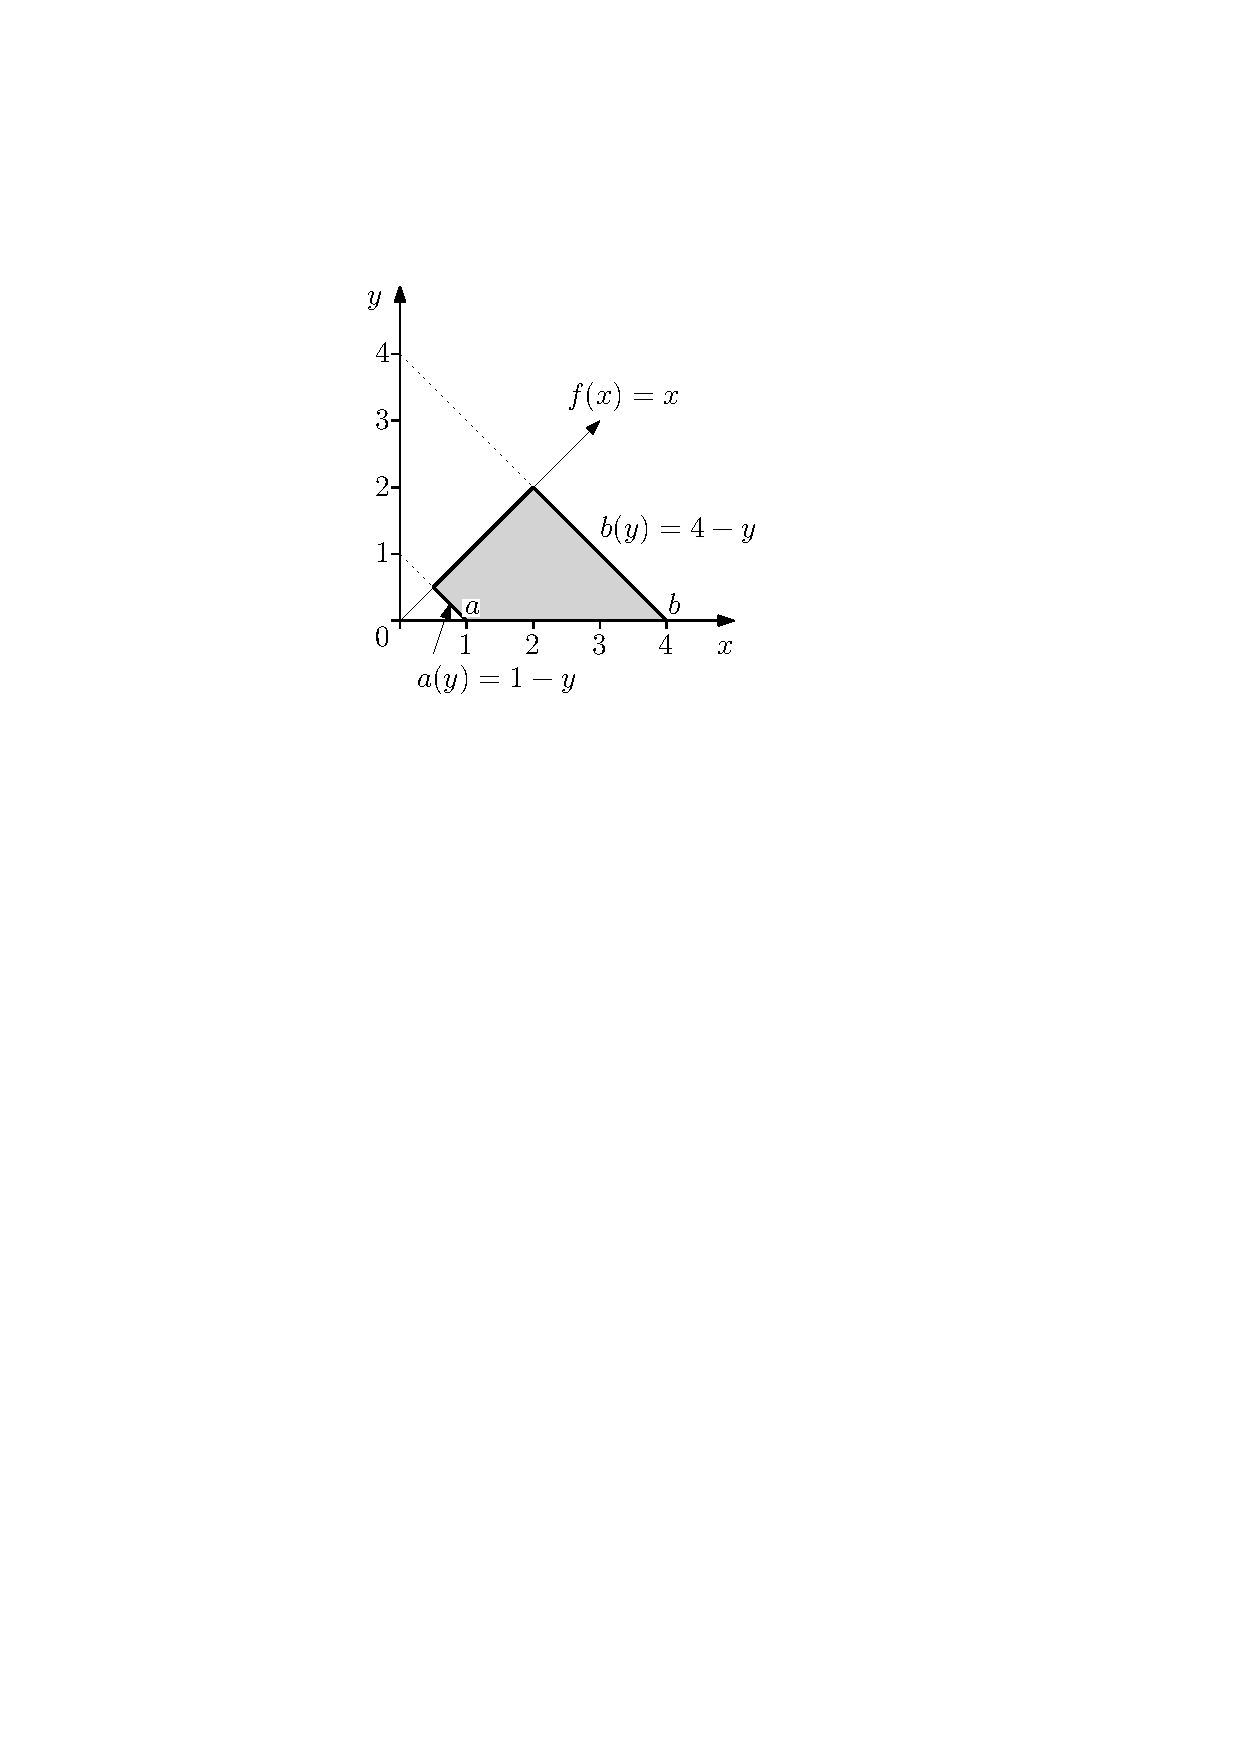
\includegraphics[width=0.3\textwidth]{fig12}
%\caption{Region bounded by the $x$-axis and the lines $f(x)=x$, $a(y)=1-y$, and $b(y)=4-y$. Reproduced from Quaestiones Mathematicae (2012) 35: 265-296 with permission \copyright~ NISC (Pty) Ltd.}
%\label{fig:ex1}
%\end{figure}
\begin{figure}[htb]
\centering
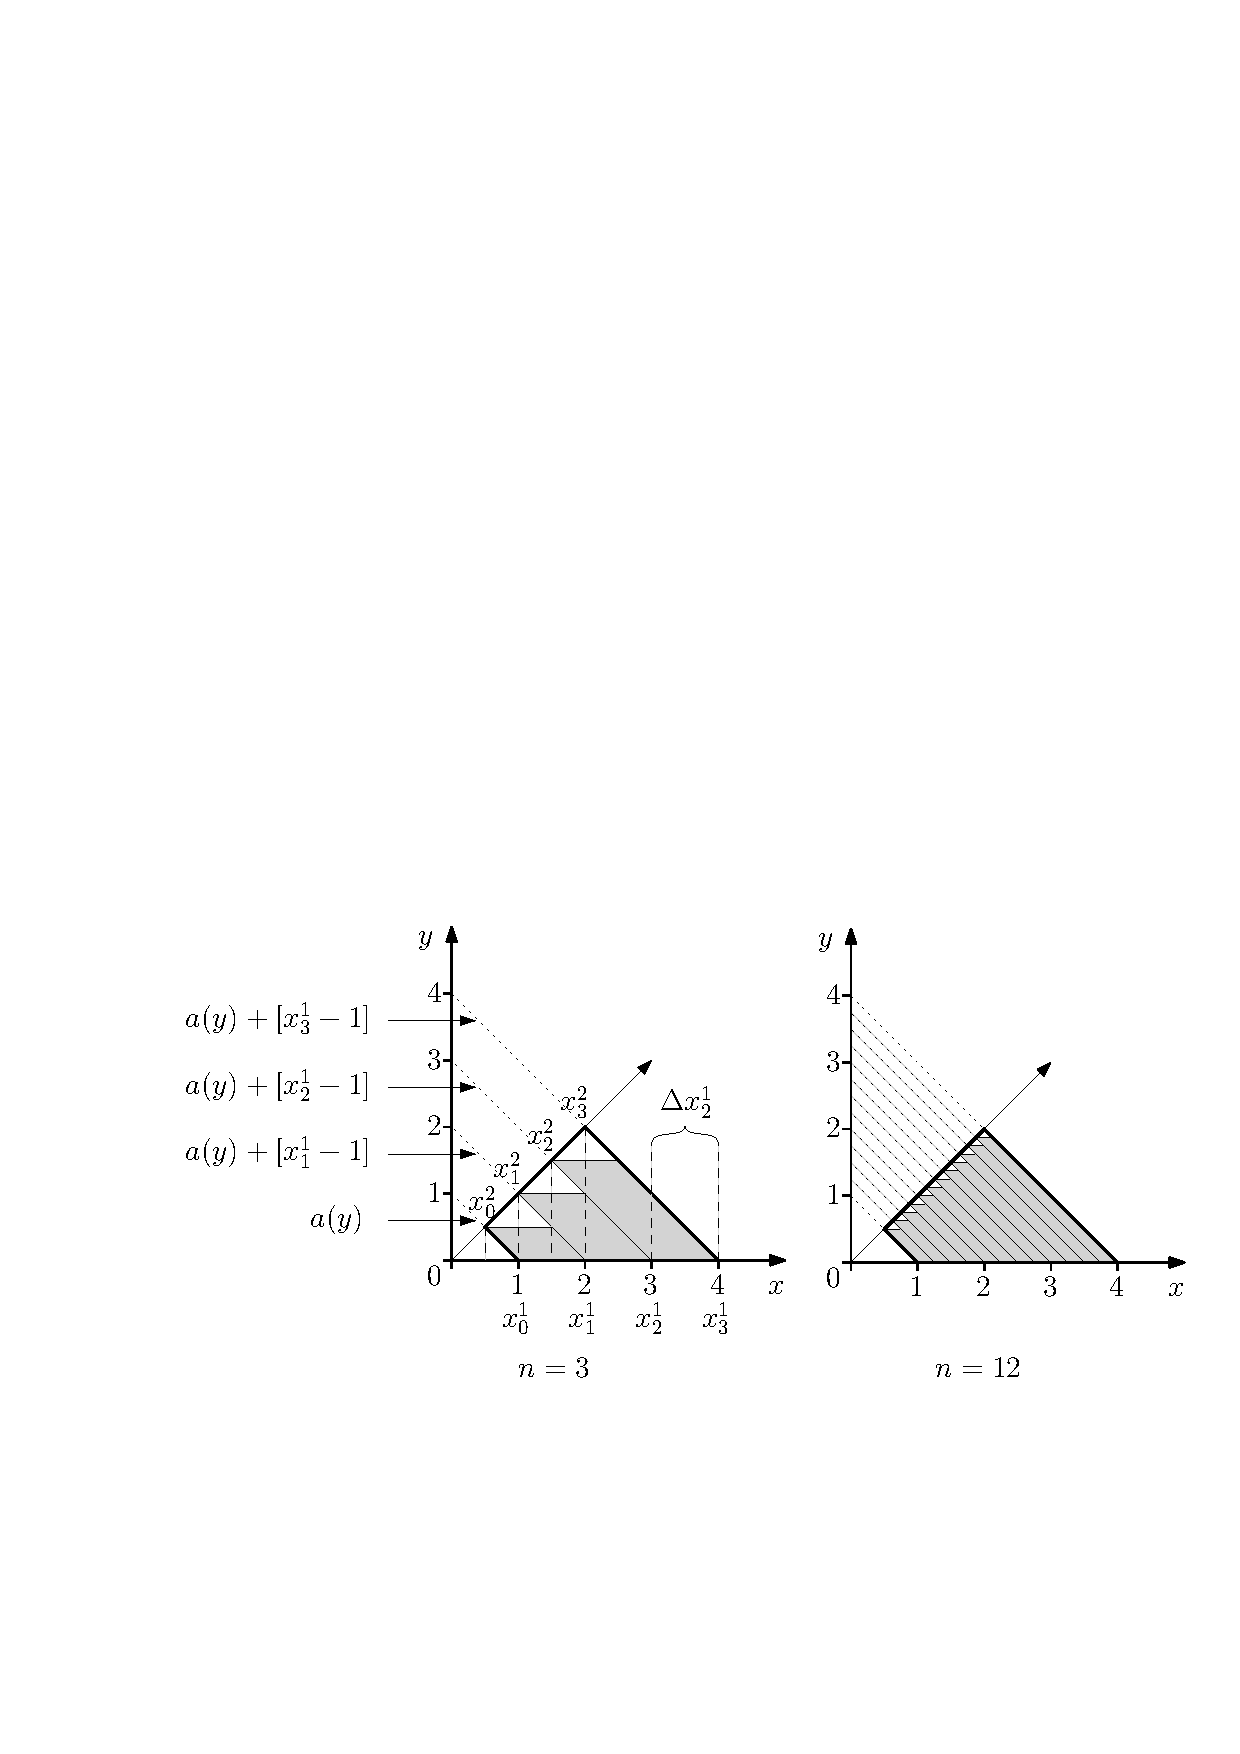
\includegraphics[width=0.75\textwidth]{fig13.pdf}
\caption{Region bounded by the $x$-axis and the lines $f(x)=x$, $a(y)=1-y$, and $b(y)=4-y$. In the case of $R$: $a=1$, $b=4$, $a'=\frac{1}{2}$ and $b'=2$. The figure also depicts the partition points $x_i^2$ as used in the Cavalieri sum (see Equation~\eqref{eq:cav_sum}). Reproduced from Quaestiones Mathematicae (2012) 35: 265-296 with permission \copyright~ NISC (Pty) Ltd.}
\label{fig:caval2}
\end{figure}

%\noindent
%The area of $R$ can be determined as follows if we employ the classical notion of integration:
%\begin{equation}
%\int_0^2x\, dx+\int_2^44-x\, dx- \int_0^{\frac{1}{2}}x\, dx-\int_{\frac{1}{2}}^11-x\, dx = 3.75. 
%\end{equation}

The area of $R$ can be approximated by summing together the area of rectangular integrations strips that inscribe $R$. There, however, exist a more 
straightforward way in which we can approximate the area of $R$: we can sum together the area of non-rectangular integration strips inscribing $R$. This alternative approach 
will only succeed it the sides of the aforementioned integration strips are all tranlsations of the function $a(y)$. 

Let us express this idea more formally. Let $(x_i^1)_{i=0}^{n}$ denote a partition on the $x$-axis, such that $a = x_0^1 < x_1^1 < \cdots < x_n^1 = b$, and $\Delta x_i^1 = x_{i+1}^1 - x_i^1$.
We are now able to construct the following lower Cavalieri sum (Equation~\ref{eq:c_low}):
\begin{equation}
\label{eq:cav_sum}
\sum_{i=0}^{n-1} f(x_i^2)\Delta x_i^1.
\end{equation}
The partition points $(x_i^2)_{i=0}^{n}$ are depicted in Fig.~\ref{fig:caval2}. Cavalieri's principle tells us that the area of integration strip $i$ is equal to $f(x_i^2)\Delta x_i^1$. Equation.~\eqref{eq:cav_sum}, therefore, approximates the area of $R$. In the limit Eq.~\eqref{eq:cav_sum} approaches 
the Cavalieri integral (Definition~\ref{def:cav_integral}):
\begin{equation}
\label{eq:caval1}
\int_{a(y)}^{b(y)}f(x)\, dx = \lim_{n\to \infty}\sum_{i=0}^{n-1} f(x_i^2)\Delta x_i^1.
\end{equation}
It is, however, quite hard to evaluate the above integral directly. Fortunately, it is easy to convert a Cavalieri integral into an equivalent Riemann or Riemann-Stieltjes 
integral by using the functions $h$ and $g$ (Theorem~\ref{t:conv}). Expressed mathematically:
\begin{equation}
\label{eq:main_cav}
\int_{a(y)}^{b(y)}f(x)\,dx =\int_a^b f \circ h (x)\, dx = \int_{a'}^{b'} f(x) dg(x).
\end{equation}
We can calculate $g$ as follows (Definition~\ref{def:g}):
\begin{equation}
g(x) = x - a\circ f(x) + a.
\end{equation}
Moreover, $h=g^{-1}$ (Theorem~\ref{t:inv}). We can now evaluate the Cavalieri integral by using its equivalent Riemann or Rieman-Stieltjes integral.
If we use its Riemann equivalent we obtain:
\begin{equation}
\int_{a(y)}^{b(y)}f(x)\, dx = \int_a^b f \circ h (x)\, dx = \dfrac{1}{2}\int_1^4x\, dx = 3.75.  
\end{equation}
If we use its Riemann-Stieltjes equivalent we obtain:
\begin{equation}
\int_{a(y)}^{b(y)}f(x)\, dx = \int_{a'}^{b'} f \, dg(x) = \int_{\frac{1}{2}}^2x\, d2x = 3.75.  
\end{equation}

\noindent
Conversely, if $g$ is known (and not $a(y)$) and $g(a') = a$ then we can calculate $a(y)$ using the following \cite{grobler19}:
\begin{equation}
\label{eq:a_y}
a(y) = f^{-1}(y) - g\circ f^{-1}(y) + g(a'). 
\end{equation}
Eq.~\eqref{eq:a_y} allows us to transform a Riemann-Stieltjes integral into an equivalent Cavalieri integral. 
Furthermore, this transformation enables us to assign a geometric interpretation to a Riemann-Stieltjes integral. The interpretation being:
it represents the area obtained by summing together the area of an infinite number of non-rectangular infinitesimals; all of them being translations of $a(y)$. Note,
$b(y) = a(y) + (b-a)$.

 
 
 
 
 
 
 
%%%%%%%%%%%%%%%%%%%%%%%%%%%%%%%%%%%%%%%%%%%%%%%%%
\section*{Acknowledgements}

 The author thanks his institution for the support, under Grant No ...

%%%%%%%%%% References %%%%%%%%%%%%%%%%%%%%%%%%%%%%%%%%
%%%% arranged in ALPHABETIC ORDER of Authors' Families
%%%% for articles, insert also DOI numbers if available

 \begin{thebibliography}{99}
 \normalsize

%%%% example for a book %%%%%%%%%%%%%

\bibitem{GasRah}
 G. Gasper, M. Rahman,
 \emph{Basic Hypergeometric Series}.
 Cambridge University Press, Cambridge (1990).

%%%% example for article in FCAA journal %%%%%%%%%%%%%%%%%

\bibitem{Kir}
 V. Kiryakova,
 A brief story about the operators of generalized
fractional calculus.
 \emph{Fract. Calc. Appl. Anal.} \textbf{11}, No 2 (2008), 201--218; DOI: ..........

%%%% example for journal's article %%%%%%%%%%%%%%%%%

\bibitem{Moak}
 D.S. Moak,
 The $q$-analogue of the Laguerre polynomials.
\emph{J. Math. Anal. Appl.} \textbf{81}, No 1 (1981), 20--47. % ; doi: ........

%%%% example for a paper in Proceedings %%%%%%%%%%%%%

\bibitem{Rosbl}
 M. Rosenblum,
 Generalized Hermite polynomials and the Bose-like oscillator
 calculus.
 In: \emph{Operator Theory: Advances and Applications},
 Birkh\"auser, Basel (1994), 369--396.
%%%%%%%%%%%%%%%%%%%%%%%%%%%%%%%%%%%%%%%%%%%%%%%%%%%%

\end{thebibliography} %%%%%%%%%%%%%%%%%%%%%%%%%%%%%%%%

%%%%%%%%%% put authors' addresses here, in \it %%%%%%%%

 \bigskip \smallskip

 \it

 \noindent
   %(First) Author's full postal address
$^1$ Institute of Mathematics and Informatics \\
Bulgarian Academy of Sciences \\
"Acad. G. Bontchev" Str., Block 8 \\
Sofia -- 1113, BULGARIA  \\[4pt]
  e-mail: virginia@diogenes.bg
\hfill Received: November 1, 2014 \\[12pt]
  % Second Author's address
$^2$ Dept. of Physics, University of Bologna\\
Via Irnerio 46, I -- 40126 Bologna, ITALY \\[4pt]
  e-mail: .....

\end{document} %%%%%%%%%%%%%%%%%%%%%%%%%%%%%%%%%%%%%
